\chapter{Experiments on MNIST}

Na początek chciałbym zacząć od odtworzenia docelowego problemu na prostszych danych jakim jest zbiór MNIST. Pozwoli to w ogólności stwierdzić sensowność skorzystania z wybranego modelu. Zakładam, że jeśli eksperyment nie powiódłby się na łatwiejszych danych, to raczej nie powiedzie się również na tych bardziej skomplikowanych. To miejsce traktuje jako poligon testowy. Pozwoli mi to też nabrać pewnego rodzaju doświadczenia z wybranym modelem.

Sytuację, którą będę chciał poddać testowi jest całkowite niezbalansowanie danych, a wręcz brak danych drugiej kategorii i obserwacja jak zachowuje sie w takim przypadku model. Będę chciał to osiągnąć poprzez uczenie modelu jedynie na danych pochodzących z dwóch klas [4, 7], a następnie obserwacja tego co się stanie z modelem przy zaaplikowania danych z klasy [5]. Ma to odtworzyć sytuację gdzie danych opisujących zmiany nowotworowe jest przytłaczająco mniej od tych zdrowych.

\section{MNIST}

Jest to zbiór po kategoryzowanych odręcznie napisanych cyfr. Wszystkie obrazki są czarno-białe, rozmiaru 28x28 i wycentrowane. Każdy piksel ma wartość dualną: 0 albo 1. Zbiór składa się z 60000 danych treningowych i 10000 testowych. Przykładowe obrazki \ref{fig:mnist}.

\begin{figure}[h!]
    \centering
    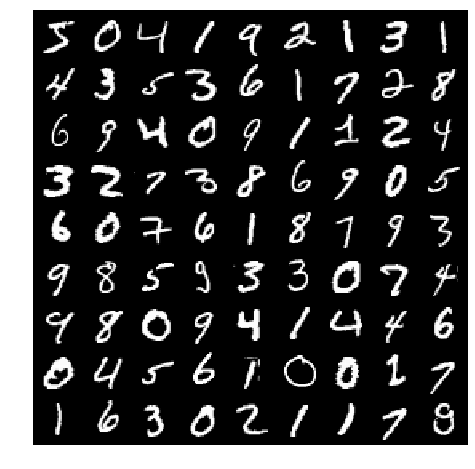
\includegraphics[width=0.4\textwidth]{images/mnist}
    \caption{Samples from MNIST dataset}
    \label{fig:mnist}
\end{figure}

\section{VAE}

Na rysunku \ref{fig:vae} znajduje się efekt wyuczenia modelu VAE z warstwą ukrytą rozmiaru 20. Po lewej widać rekonstrukcje, a po prawej efekty zdekodowania wektora wygenerowanego ze standardowego rozkładu normalnego.

\begin{figure}[h!]
  \centering
  \begin{subfigure}[b]{0.57\linewidth}
    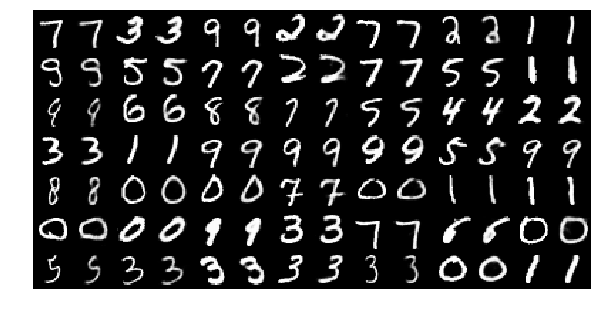
\includegraphics[width=\linewidth]{images/mnist_recon}
    \caption{W nieparzystych kolumnach znajdują się oryginalne obrazki, natomiast po prawej ich rekonstrukcje}
  \end{subfigure}
  \begin{subfigure}[b]{0.30\linewidth}
    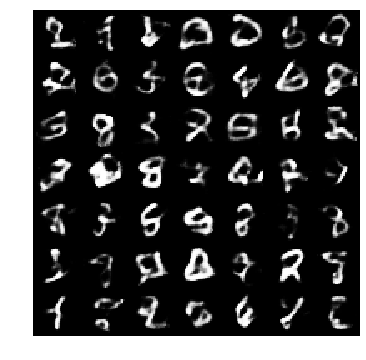
\includegraphics[width=\linewidth]{images/mnist_gen}
    \caption{Przykłady wygenerowanych obrazków}
  \end{subfigure}
  \caption{Przedstawienie efektów modelu VAE}
  \label{fig:vae}
\end{figure}

Dodatkowo warto byłoby zobaczyć jak konkretne cyfry rozrzucane są w przestrzeni. 20 wymiarów jest dosyć trudne do zwizualizowania, więc wyuczyłem model dla reprezentacji ukrytej rozmiaru 2. Na rysunku \ref{fig:mnist_2d} znajdują sie wyniki. Wartym odnotowania jest fakt, że niektóre klasy są bardzo dobrze separowalne. Widać tu właśnie opisane wcześniej zalety modelu VAE. Te ciekawą własność wyniku reprezentacji będę chciał wykorzystać w późniejszej analizie.

\begin{figure}[h!]
    \centering
    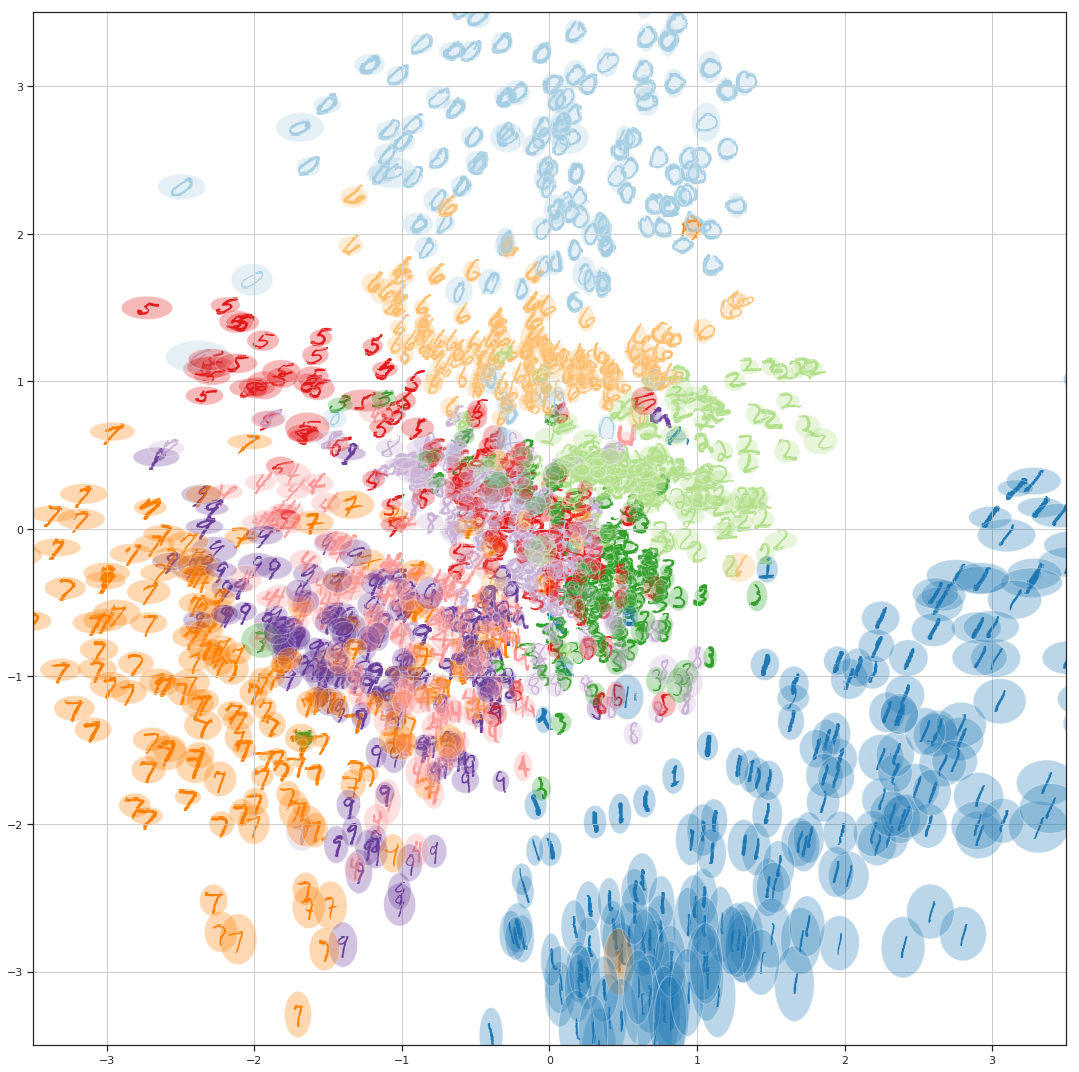
\includegraphics[width=1.\textwidth]{images/mnist_2d}
    \caption{}
    \label{fig:mnist_2d}
\end{figure}

W oryginalnym problemie mamy bardzo duży dysonans pomiędzy ilością przykładów dla każdej z klas. Według statystyk dane z komórkami rakowymi stanowią ~1\% wszystkich. Ciężko jest wiec nawet mówić o jakimś sensownym podejściu supervised. Do zasymulowania tego problemu dla MNIST będę uczył model jedynie na dwóch klasach [4, 7], a następnie testował zachowanie reprezentacji ukrytej dla przekładów z klasy 5.

Rozmiar reprezentacji ukrytej wynosi 10. Analizować natomiast będziemy 2 składowe kosztu dla modelu VAE: KLD oraz błąd rekonsrukcji MSE. Na rysunku \ref{fig:mnist_compare} znajduje się przedstawienie ich wraz z histogramami. Można zauważyć, że wyłącznie na podstawie samego błędu rekonstrukcji można z bardzo dużą dokładnością określić dane pochodzące z klasy 5, mimo iż model nie widział żadnych ich przykładów podczas uczenia.

\begin{figure}[h!]
    \centering
    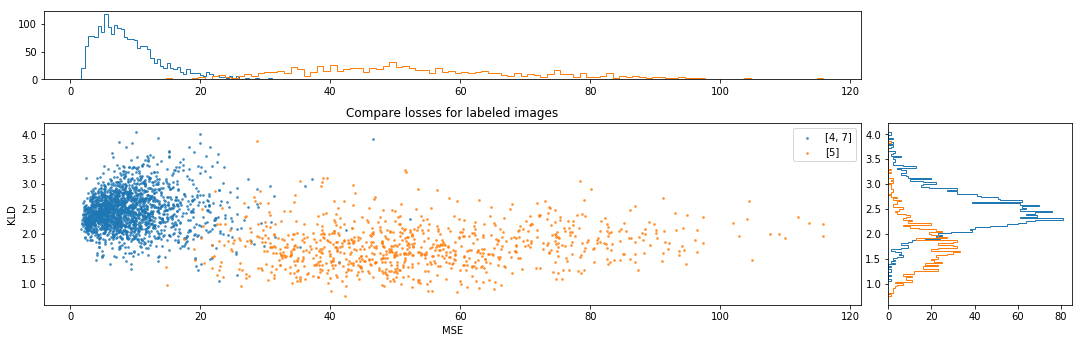
\includegraphics[width=1.0\textwidth]{images/mnist_compare}
    \caption{}
    \label{fig:mnist_compare}
\end{figure}

Do określenia jak rzeczywiście dobra jest ta separacja można wykorzystać krzywą ROC. Traktujemy to jako problem binarnej klasyfikacji, gdzie dane z klasy 5 będą oznaczone jako 1, a z [4, 7] jako 0. Wartość confidence to suma kosztów KLD i MSE. Jak widać na rysunku \ref{fig:mnist_roc} takie podejście osiąga prawie 100\% skuteczność. Podobne podejście będę chciał zastosować do danych medycznych.

\begin{figure}[h!]
    \centering
    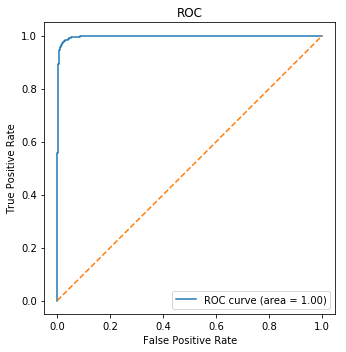
\includegraphics[width=0.5\textwidth]{images/mnist_roc}
    \caption{}
    \label{fig:mnist_roc}
\end{figure}

\subsection{Krzywa ROC i AUC}

Krzywa ROC (Receiver Operating Characteristic) jest narzędziem do oceny poprawności klasyfikatora binarnego. Bazuje ona na wyliczaniu charakterystyki jakościowej modelu predykcji w wielu różnych punktach odcięcia. Z praktycznego punktu widzenia działa to na takiej zasadzie, że mamy dane pochodzące z dwóch klas. Model odpowiada z jaką pewnością dane należą do klasy 1. Następnie badamy różne progi i klasyfikujemy obiekty (jeśli przewidziana wartość jest powyżej progu to 1 wpp 0). Dla uzyskanych klasyfikacji liczymy TPR oraz FPR i nanosimy te wartości na wykres. Warto zauważyć, że dla losowego modelu jego wykres to prosta przechodząca przez (0, 0) i (1, 1). Dzieje się tak, ponieważ w przy każdym progu połowa danych będzie nad i połowa pod. Idealny model znajduje się w punkcie (0, 1).

Przydatne jest również obliczenie pola powierzchni pod krzywą AUC (Area Under Curve). Interpretuje się ją jako prawdopodobieństwo, że badany model predykcyjny oceni wyżej losowy element klasy pozytywnej od losowego elementu klasy negatywnej.

\section{Deep feature consistent variational auto-encoder}

Podobny eksperyment jw. przeprowadziłem również dla modelu DFC. Na początku jednak warto zobaczyć co zyskujemy na zmianie podejścia do kosztu rekonstrukcji. Różnice prezentują się na rysunku \ref{fig:vae_dfc_recon}. Widać, że rekonstrukcje są mniej rozmazane niż przy standardowym VAE. Dodatkowo lepiej rekonstruuje takie elementy jak np. pozioma kreska w cyfrze 7. 

\begin{figure}[h!]
    \centering
    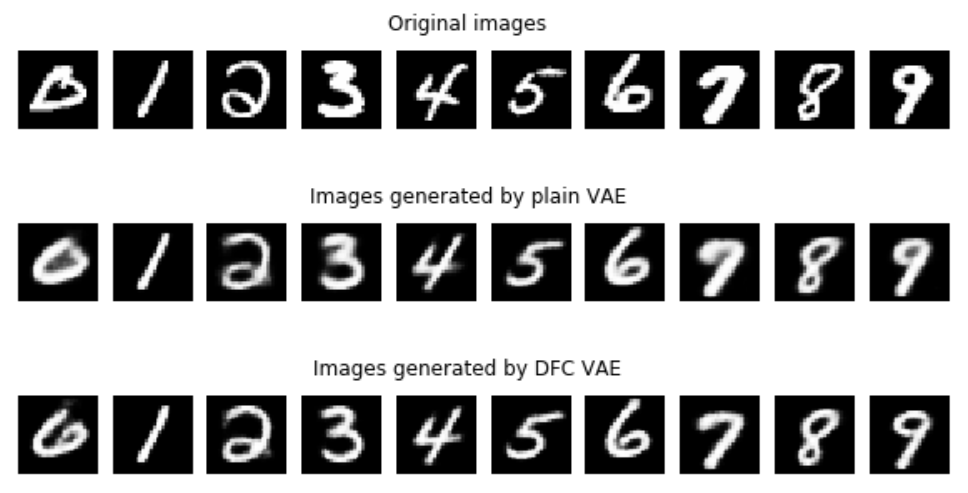
\includegraphics[width=0.8\textwidth]{images/vae_dfc_gen}
    \caption{}
    \label{fig:vae_dfc_recon}
\end{figure}

Na rysunku \ref{fig:dfc_mnist_compare} przedstawiony jest efekt przeprowadzenia analogicznego eksperymentu z nauką na jedynie przykładach z klas [4, 7] i sprawdzeniu zachowania dla danych z klasy 5. Zamiast kosztu rekonstrukcji MSE używamy błędu perceptualnego. Dodatkowy model splotowy również nie widział danych pochodzących z 5 klasy. Jak widać separacja jest co najmniej tak dobra jak w przypadku zwykłego VAE.

\begin{figure}[h!]
    \centering
    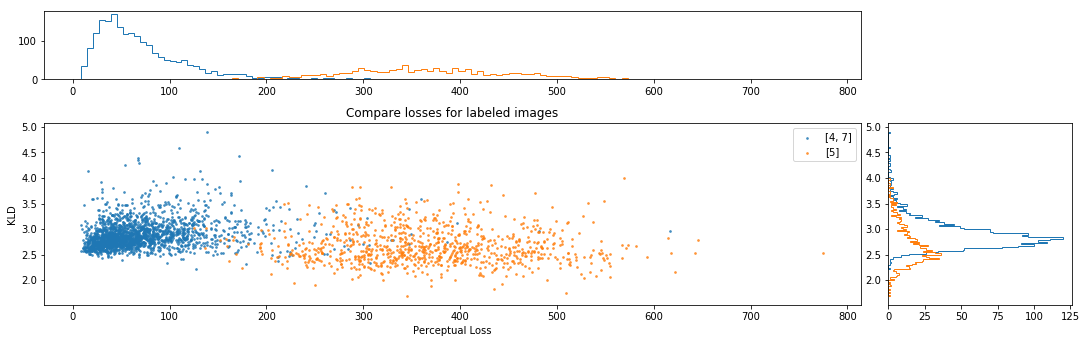
\includegraphics[width=1.0\textwidth]{images/dfc_mnist_compare}
    \caption{}
    \label{fig:dfc_mnist_compare}
\end{figure}
